\documentclass{article}
\usepackage{graphicx}
\usepackage{amsmath}
\usepackage{pgfplots}
\usepackage{physics}
\usepackage{cancel}
\usepackage{enumitem}
\usepackage{txfonts}

\pgfplotsset{compat=1.18}

\usepackage[a4paper, top=1cm, bottom=2cm, left=2cm, right=2cm, includehead, includefoot]{geometry}

\begin{document}

\noindent
Physics 4A - Classical Mechanics \hfill Prof. Roger King

\noindent\rule{\textwidth}{0.4pt}

\begin{center}
    \textbf{\LARGE Homework 8} \\
    \vspace{12pt}
    \large Aaron W. Tarajos \\
    \textit{\today}
\end{center}

\noindent\rule{\textwidth}{0.4pt}

\section*{Problem 1}
A 0.315-kg particle moves from an initial position $\va{r}_1 = 2.00\ \vu{i} - 1.00\ \vu{j} + 3.00\ \vu{k}$ m to a final position $\va{r}_2 = 4.00\ \vu{i} - 3.00\ \vu{j} - 1.00\ \vu{k}$ m while a force $\va{F} = 2.00\ \vu{i} - 3.00\ \vu{j} + 1.00\ \vu{k}$ N acts on it. What is the work done by the force on the particle?

\subsection*{Solution}
The distance traveled by the particle, $\va{d}$, is equal to the difference in final and initial position
\begin{align*}
	\va{d} &= \va{r_2} - \va{r_1} \\
	       &= \left( 4.00 - 2.00 \right)\ \vu{i} + \left( -3.00 + 1.00 \right)\ \vu{j} + \left( -1.00 -3.00 \right)\ \vu{k} \\
	       &= 2.00\ \vu{i} - 2.00\ \vu{j} - 4.00\ \vu{k}
\end{align*}
Then work is the dot product of $\va{F}$ and $\va{d}$
\[
	W = \va{F} \cdot \va{d} = (2)(2) + (-2)(-3) + (-4)(1) = \boxed{6\ \text{J}}
\]

\section*{Problem 2}
Compute the kinetic energy for each of the cases below. Through what distance would a 800-N force have
to act to stop each object? \\
(a) A 150-g baseball moving at 40 m/s; \\
(b) a 13-g bullet from a rifle moving at 635 m/s; \\
(c) a 1500-kg Corvette moving at 250 km/h; \\
(d) a $1.8 \times 10^5$-kg Concorde airliner moving at 2240
km/h.

\subsection*{Solution}
The kinetic energy is given by

\begin{equation}
	k = \frac{1}{2}mv^2
\end{equation}
Then

\[
	k = Fd \implies d = \frac{k}{F}
\]
Using these equations to solve for each part;
\subsubsection*{Part a:}
\[
	k = \frac{1}{2} (0.150)(40)^2 = \boxed{120\ \text{J}}
\]
and

\[
	d = \frac{120}{800} = \boxed{0.15\ \text{m}}
\]

\subsubsection*{Part b:}
\[
	k = \frac{1}{2} (0.013)(635)^2 = \boxed{2620.96\ \text{J}}
\]
and

\[
	d = \frac{2620.96}{800} = \boxed{3.276\ \text{m}}
\]

\subsubsection*{Part c:}
\[
	k = \frac{1}{2} (1500)(69.44444)^2 = \boxed{3\ 616\ 897\ \text{J}}
\]
and

\[
	d = \frac{3\ 616\ 897}{800} = \boxed{4.521\ \text{km}}
\]

\subsubsection*{Part d:}
\[
	k = \frac{1}{2} (1.8 \times 10^5)(622.2222)^2 = \boxed{3.484\times10^{10}\ \text{J}}
\]
and

\[
	d = \frac{2620.96}{800} = \boxed{43\ 555.552\ \text{km}}
\]


\section*{Problem 3}
Compute the kinetic energies for each of the following. What force would be required to stop each object in
1.00 km? \\
(a) The $8.00 \times 10^7$-kg carrier Nimitz moving at 55 km/h; \\
(b) a $3.4 \times 10^5$-kg Boeing 747 moving at 1000 km/h; \\
(c) the 270-kg Pioneer 10 spacecraft moving at 51,800 km/h.

\subsection*{Solution}
\subsubsection*{Part a:}
Kinetic energy is

\[
	k = \frac{1}{2} mv^2 = \frac{1}{2}(8.00 \times 10^7)(15.27778)^2 = \boxed{9.336\times10^{9}\ \text{J}}
\]
and the force required to stop it is

\[
	F = \frac{9.336\times10^{9}\ \text{J}}{1000\ \text{m}} = \boxed{9\ 336\ 422\ .\ 469\ \text{N}}
\]

\subsubsection*{Part b:}
Kinetic energy is

\[
	k = \frac{1}{2}(3.4 \times 10^5)(277.7778)^2 = \boxed{1.312\times10^{10}\ \text{J}}
\]
and the force required to stop it is

\[
	F = \frac{1.312\times10^{10}\ \text{J}}{1000\ \text{m}} = \boxed{13\ 117\ 286\ .\ 049\ \text{N}}
\]

\subsubsection*{Part c:}
Kinetic energy is

\[
	k = \frac{1}{2}(3.4 \times 10^5)(277.7778)^2 = \boxed{1.312\times10^{10}\ \text{J}}
\]
and the force required to stop it is

\[
	F = \frac{1.312\times10^{10}\ \text{J}}{1000\ \text{m}} = \boxed{13\ 117\ 286\ .\ 049\ \text{N}}
\]

\section*{Problem 4}
A 1.50-kg block is moved at constant speed in a vertical plane from position 1 to position 3 via several
routes shown in the figure. Compute the work done by gravity on the block for each segment indicated,
where $W_{ab}$ means work done from a to b. \\
(a) $W_{1\ 3}$ \\
(b) $W_{1\ 2} + W_{2\ 3}$ \\
(c) $W_{1\ 4} + W_{4\ 3}$ \\
(d) $W_{1\ 4} + W_{4\ 5} + W_{5\ 3}$

\begin{figure}[ht]
    \centering
    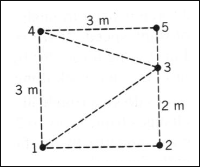
\includegraphics[scale=.5]{drawing-1.png}
\end{figure}

\subsection*{Solution}
\subsubsection*{Part a:}
Let $\va{d}$ be the path from position 1 to position 3, the angle between $\va{F}_g$ and $\va{d}$ is given by
\[
	\phi_g = 90 + \arctan\left(\frac{d_y}{d_x}\right)
\]
then

\[
	W_{1\ 3} = (mg)(d)\cos \phi_g
\]
substituting the given values values
\[
	W_{1\ 3} = (1.50)(9.81)(\sqrt{13}) \cos \left( 90 + \arctan \left( \frac{2}{3} \right) \right) = \boxed{-29.43\ \text{J}}
\]

\subsubsection*{Part b:}
The distance vector $\va{d}$ is orthogonal to $\va{F}_g$ for $W_{1\ 2}$, therefore that component is zero. For $W_{2\ 3}$, the angle between the $\va{F_g}$ and $\va{d}$ is $180^\circ$ so we have
\[
	W_{1\ 2} + W_{2\ 3} = 0 + (mg)(d)(-1) = (1.50)(9.81)(2)(-1) = \boxed{-29.43\ \text{J}}
\]

\subsubsection*{Part c:}
Similar to part a, we have;
\[
	\phi_g = 90 - \arctan\left(\frac{d_y}{d_x}\right)
\]
for $W_{4\ 3}$, giving us

\begin{align*}
	W_{1\ 4} + W_{4\ 3} &= (mg)(d_1)(-1) + (mg)(d_2)\left(cos\left( 90 - \arctan\left(\frac{d_y}{d_x}\right) \right) \right) \\
			    &= (1.50 \cdot 9.81)(3)(-1) + (1.50 \cdot 9.81)(\sqrt{10})\left(cos\left( 90 - \arctan\left(\frac{1}{3}\right) \right) \right) \\
			    &= \boxed{-29.43\ \text{J}}
\end{align*}


\subsubsection*{Part d:}
This is similar to part b, except, for the third component of work, $\phi_g = 0$.
\[
	W_{1\ 4} + W_{4\ 5} + W_{5\ 3} = (mg)(d)(-1) + 0  + (mg)(d)(1)= (1.5)(9.81)(3)(-1) +  (1.5)(9.81)(1)(1) = \boxed{-29.43\ \text{J}}
\]

\section*{Problem 5}
What is the work needed to lift 14.7 kg of water from a well 11.0 m deep. Assume the water has a constant
upward acceleration of 0.700 m/s$^2$.

\subsection*{Solution}
Let $\va{F}$ be the upward force acting on the bucket

\[
	\va{F} = m \va{a}
\]
then work $W$ is given by

\[
	W = Fd \cos(0) = (14.7)(0.7 + 9.81)(11) = \boxed{1699.467\ \text{J}}
\]


\section*{Problem 6}
The variation of a force with position is shown in the figure below. Find the work from
(a) $x = 0$ to $x = -A$ \\
(b) $x = +A$ to $x = 0$

\section*{Problem 7}
Consider a particle on which several forces act, one of which is known to be constant in time:
$\va{F}_1 = 3.00\ \vu{i} + 4.00\ \vu{j}$ N. As a result, the particle moves along a straight path from a Cartesian coordinate of
(0.00 m, 0.00 m) to (5.00 m, 6.00 m). What is the work done by $\va{F}_1$?

\section*{Problem 8}
A bungee cord exerts a nonlinear elastic force of magnitude $F(x) = k_1 x + k_2 x^3$, where $x$ is the distance the cord is stretched, $k_1 = 204$ N/m and $k_2 = -0.233$ N/m$^3$. How much work must be done on the cord to stretch it 16.7 m?

\end{document}
